\documentclass[11pt,a4paper]{article}
\usepackage[utf8]{inputenc}
\usepackage[english]{babel}
\usepackage{hyperref}
\usepackage{url}
\usepackage{graphicx}
\usepackage{subfig}
\usepackage{pdfpages}

\title{%
    \textbf{R \& D Workshop} \\
    Tomcat in the Cloud
    \\
    \textbf{Final Report}
}

\author{%
    Ismaïl Senhaji \\
    \small \href{mailto:ismail.senhaji@unifr.ch}{ismail.senhaji@unifr.ch} \\
    \\
    Guillaume Pythoud \\
    \small \href{mailto:guillaume.pythoud@unifr.ch}{guillaume.pythoud@unifr.ch}
    \\
    \\
    Supervised by \\
    Jean-Frederic Clere \\
    \small \href{mailto:jclere@redhat.com}{jclere@redhat.com}
}

\date{June 20, 2017}

\begin{document}
\graphicspath{{fig/}}

\maketitle

\begin{figure}[b]
    \centering
    \subfloat{
\includegraphics[height=1.5cm]{jmcs.png}}
    \\
    \subfloat{
\includegraphics[height=1.6cm]{redhat-logo.png}}
\end{figure}

\newpage
\tableofcontents

\newpage


\section{Project description}

\subsection{Project and context}

For this project, we have been assigned to \emph{Red
    Hat}\footnote{\url{http://www.redhat.com/en/about}}. Red Hat is an international
software company, specializing in open source.  Among others, they develop
the \emph{OpenShift Container
    Platform}\footnote{\url{https://www.openshift.com/container-platform/index.html}},
which is full-stack cloud management solution.

We will work on the
\emph{Tomcat}\footnote{\url{https://www.openshift.com/container-platform/index.html}}
Java web server. Our task is to extend Tomcat in order to make session
replication work in a cloud environment.

As it stands, session replication in Tomcat is not cloud ready yet. The main
issue is that it uses multicast which only works in a local network. In a cloud
deployment, instances can be distributed over the internet. This calls for the
development of a new session replication solution.


\subsection{Goals and objectives of the project}

The major goal of the project to make Tomcat's session work in the cloud. This
goal is divided in 3 steps:
\begin{enumerate}
    \item Study existing methods
    \item Implement a new solution based on one of those methods
    \item Test the implementation
\end{enumerate}

To test our implementation, we will develop a Java web application. It
will simply display these informations:

\begin{itemize}
    \item The ID of the Tomcat instance that served the request
    \item The user's session ID
    \item A counter that is incremented on every request.
\end{itemize}

A secondary goal is to build and configure a Raspberry Pi cluster, running
OpenShift. If successful, it will be presented as a demonstration at the end of
the project.

Another important goal is to provide detailed documentation for future users.
We will write a ``Quick Start Guide'' detailing the steps to follow to have a
working Tomcat cluster running in an OpenShift cloud.


\section{Methodology}

Most development will be done in Java, since Tomcat itself is written in Java.
But we suspect that most time will be spent on reading documentation and code
than on writing code.

As mentioned above, all our work is available on our GitHub repository, be it
code, documentation or simply comments and ideas.

For testing our solutions, we will use
MiniShift\footnote{\url{https://www.openshift.org/minishift/}}. MiniShift is a tool
that deploys a ``local'' (i.e\ consisting of a unique machine) OpenShift
cluster on any computer. This will allow us to run tests on our laptops, saving
the time necessary to deploy a real OpenShift installation. Only towards the
end of the project, when everything else is done, will we finally deploy our
solution on a real cluster.

\subsection{State of the art}

Our research has shown that Tomcat has two built-in session replication
solutions that could be built
on\footnote{\url{https://tomcat.apache.org/tomcat-8.5-doc/cluster-howto.html}}:

\begin{enumerate}
    \item \emph{DeltaManager}: this session manager replicates session data to
        all other instances in a cluster. Peer discovery can be either be done
        statically or dynamically. In static mode, a list of peers is hardcoded
        in Tomcat's configuration file. In dynamic mode, peers are discovered
        using multicast.

    \item \emph{PeristanceManager}: session data is stored in the filesystem or
        in a JDBC-capable database.
\end{enumerate}

Paths to explore are modifying DeltaManager to discover peer using a different
method (since multicast over the internet isn't feasible), or configure
PersistanceManager to use a distributed datastore. The first solution might be
more interesting from a performance point of view.

Finally, if none of the solutions above turn out fruitful, there still are
other paths to explore: there are solutions that bypass Tomcat's session
manager and use an external one instead. The \emph{Spring
    Framework}\footnote{\url{http://projects.spring.io/spring-framework/}} offers
such a solution, and is advertised to have built-in support for distributed
datastores such as \emph{Redis} or
\emph{Hazelcast}\footnote{\url{http://docs.spring.io/spring-session/docs/current/reference/html5/}}.
Another solution ports WildFly's session manager to
Tomcat\footnote{\url{https://github.com/wildfly-clustering/wildfly-clustering-tomcat}}.

While these solutions using external session managers are known to work, we
will mainly concentrate on those based on Tomcat, as they avoid relying on too
many external dependencies. But we consider them as a ``Plan B'' if all else
fails.


\section{Result and realization}

\subsection{Process}
As our knowledge of Tomcat was low we started by implementing a basic web application that used the built-in Tomcat solution for session replication within a cluster. We continued with this idea by developing new iteration with always new solutions for the session replication. Hence we were able to get at each iteration a better idea on how Tomcat was working and we were able to provide every time a new solution which was closest to the goal. During this process we provided different testing application that included different technology. At the beginning of the project we wanted to use Spring Boot but as it add a lot of complexity in the tomcat configuration we finally decided to not include it. All those testing applications are stored in the \emph{experiment}\footnote{\url{https://github.com/iSma/tomcat-in-the-cloud/tree/experiments}} branch in the github repository. We also discovered technologies that we eventually used in the final solution, for example \emph{fabric8 maven plugin}\footnote{\url{https://github.com/fabric8io/fabric8-maven-plugin}} that helped us build an deploy our application on Openshift.

\subsection{Testing}
To test our applications we did not implement any testing suite. As the application was simple it was quick to manually check if the requests were correctly handled. Basically we checked if the data of a selected session was correctly stored and shared on all the pods of the cluster, even after some scale up and scale down.

\subsection{Result}
The final solution we provided is inspired from \emph{Kube PING}\footnote{\url{https://github.com/jgroups-extras/jgroups-kubernetes}}, a Kubernetes discovery protocol for JGroup. We also analyzed the implementation of the multicast membership service of Tomcat and made our own membership service that used the Openshift API \footnote{\url{https://docs.openshift.com/enterprise/3.0/rest_api/index.html}} to get the running pods of the project. We also compute the alive time of each pods with the help of the \emph{creationTime} of each pods and finally add it to the membership. The implementation is described in the figure\ref{dms}. A small guide on how to use this application is specified in a \emph{Readme} file in the github repository.

\begin{figure}[h]
\centering
\caption{DynamicMembershipService}
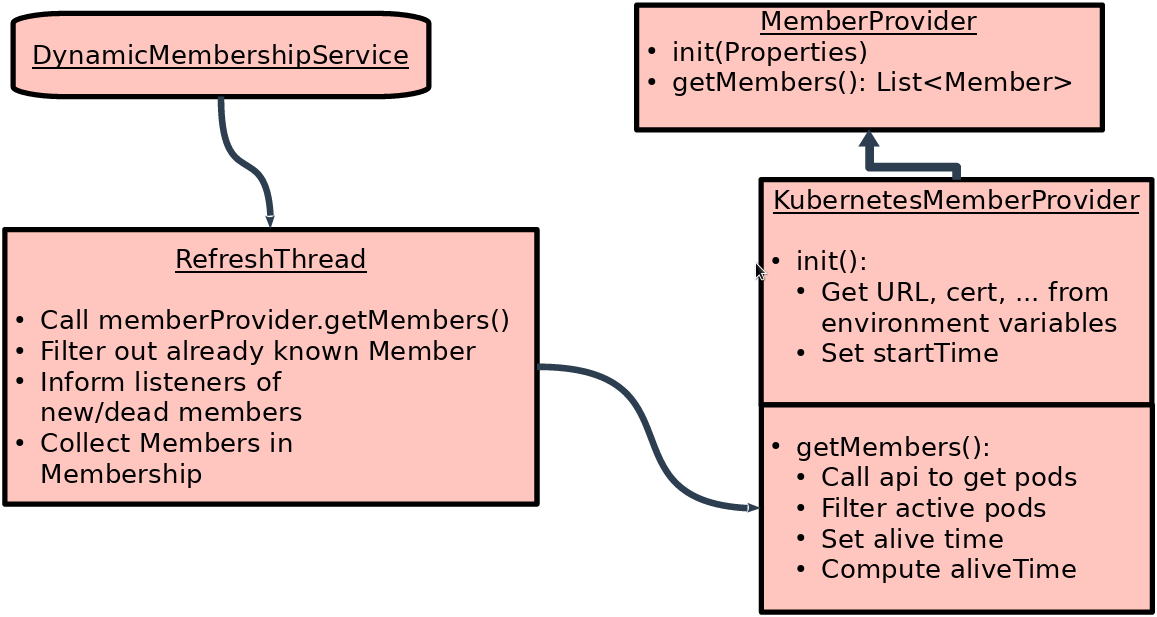
\includegraphics[width=1\textwidth]{fig/dynamicMembership}

\label{dms}
\begin{footnotesize}
Implementation of the DynamicMembershipService 
\end{footnotesize}
\end{figure}

\section{Recommendations}

\subsection{Statements of recommendations}
The solution we finally provide at the end of the project is meant to be seen as a proof of concept to help others that looks for a way of enabling session replication in an Openshift environment within a tomcat application. Hence we tried to provide a solution with the lowest possible number of dependencies and that could be easily replicated by others.

\subsection{Limitations}
As we focused on a having a working solution, our error handling is currently at bare minimum, this is something that could be improved. 
Even if the Class that call the API is called \emph{KubernetesMemberProvider} we don't know if the implementation is working on a pure Kubernetes environment as the call could differ than the one of the Openshift API.
At the moment the session data of all the pods of a namespaces/project are shared even if they are not running the same application, this could become a problem with a large scale project with multiple applications running.

\subsection{Outstanding issues and perspective for future work}
Our tests was quite simple, so developing a testing tools for session data replication checking within a cluster could be a great future step. It would provide us a best way to test our implementation and maybe find new issues that our previous testing phases did not show up.



\end{document}
